\section{Statistical laws differentiate by tissue}
Considering the GTEx dataset of healthy samples it is possible to study differences in tissues;~\cite{mele2014} suggests some approaches.

First of all, it could be interesting to study which is the fraction of transcriptome that can be explained by a certain number of genes.
To do this, it is necessary to get all the samples of a given tissue. Then one estimates the average expression per each component (gene). At this point, one has the average abundance of each gene in a tissue, dividing by the sum of all the components it is possible to obtain the fraction of the total counts in the tissue due to each gene. Sorting from greater to smaller and integrating (cumulative summing) one have the fraction of transcript due to $1, 2, 3\dots$ genes. This is reported in figure~\ref{fig:structure/gtex/fraction_of_trascriptome}. This analysis is done using TPM to avoid biases due to gene lengths or to samples sizes.
\begin{figure}[htb!]
  \centering
  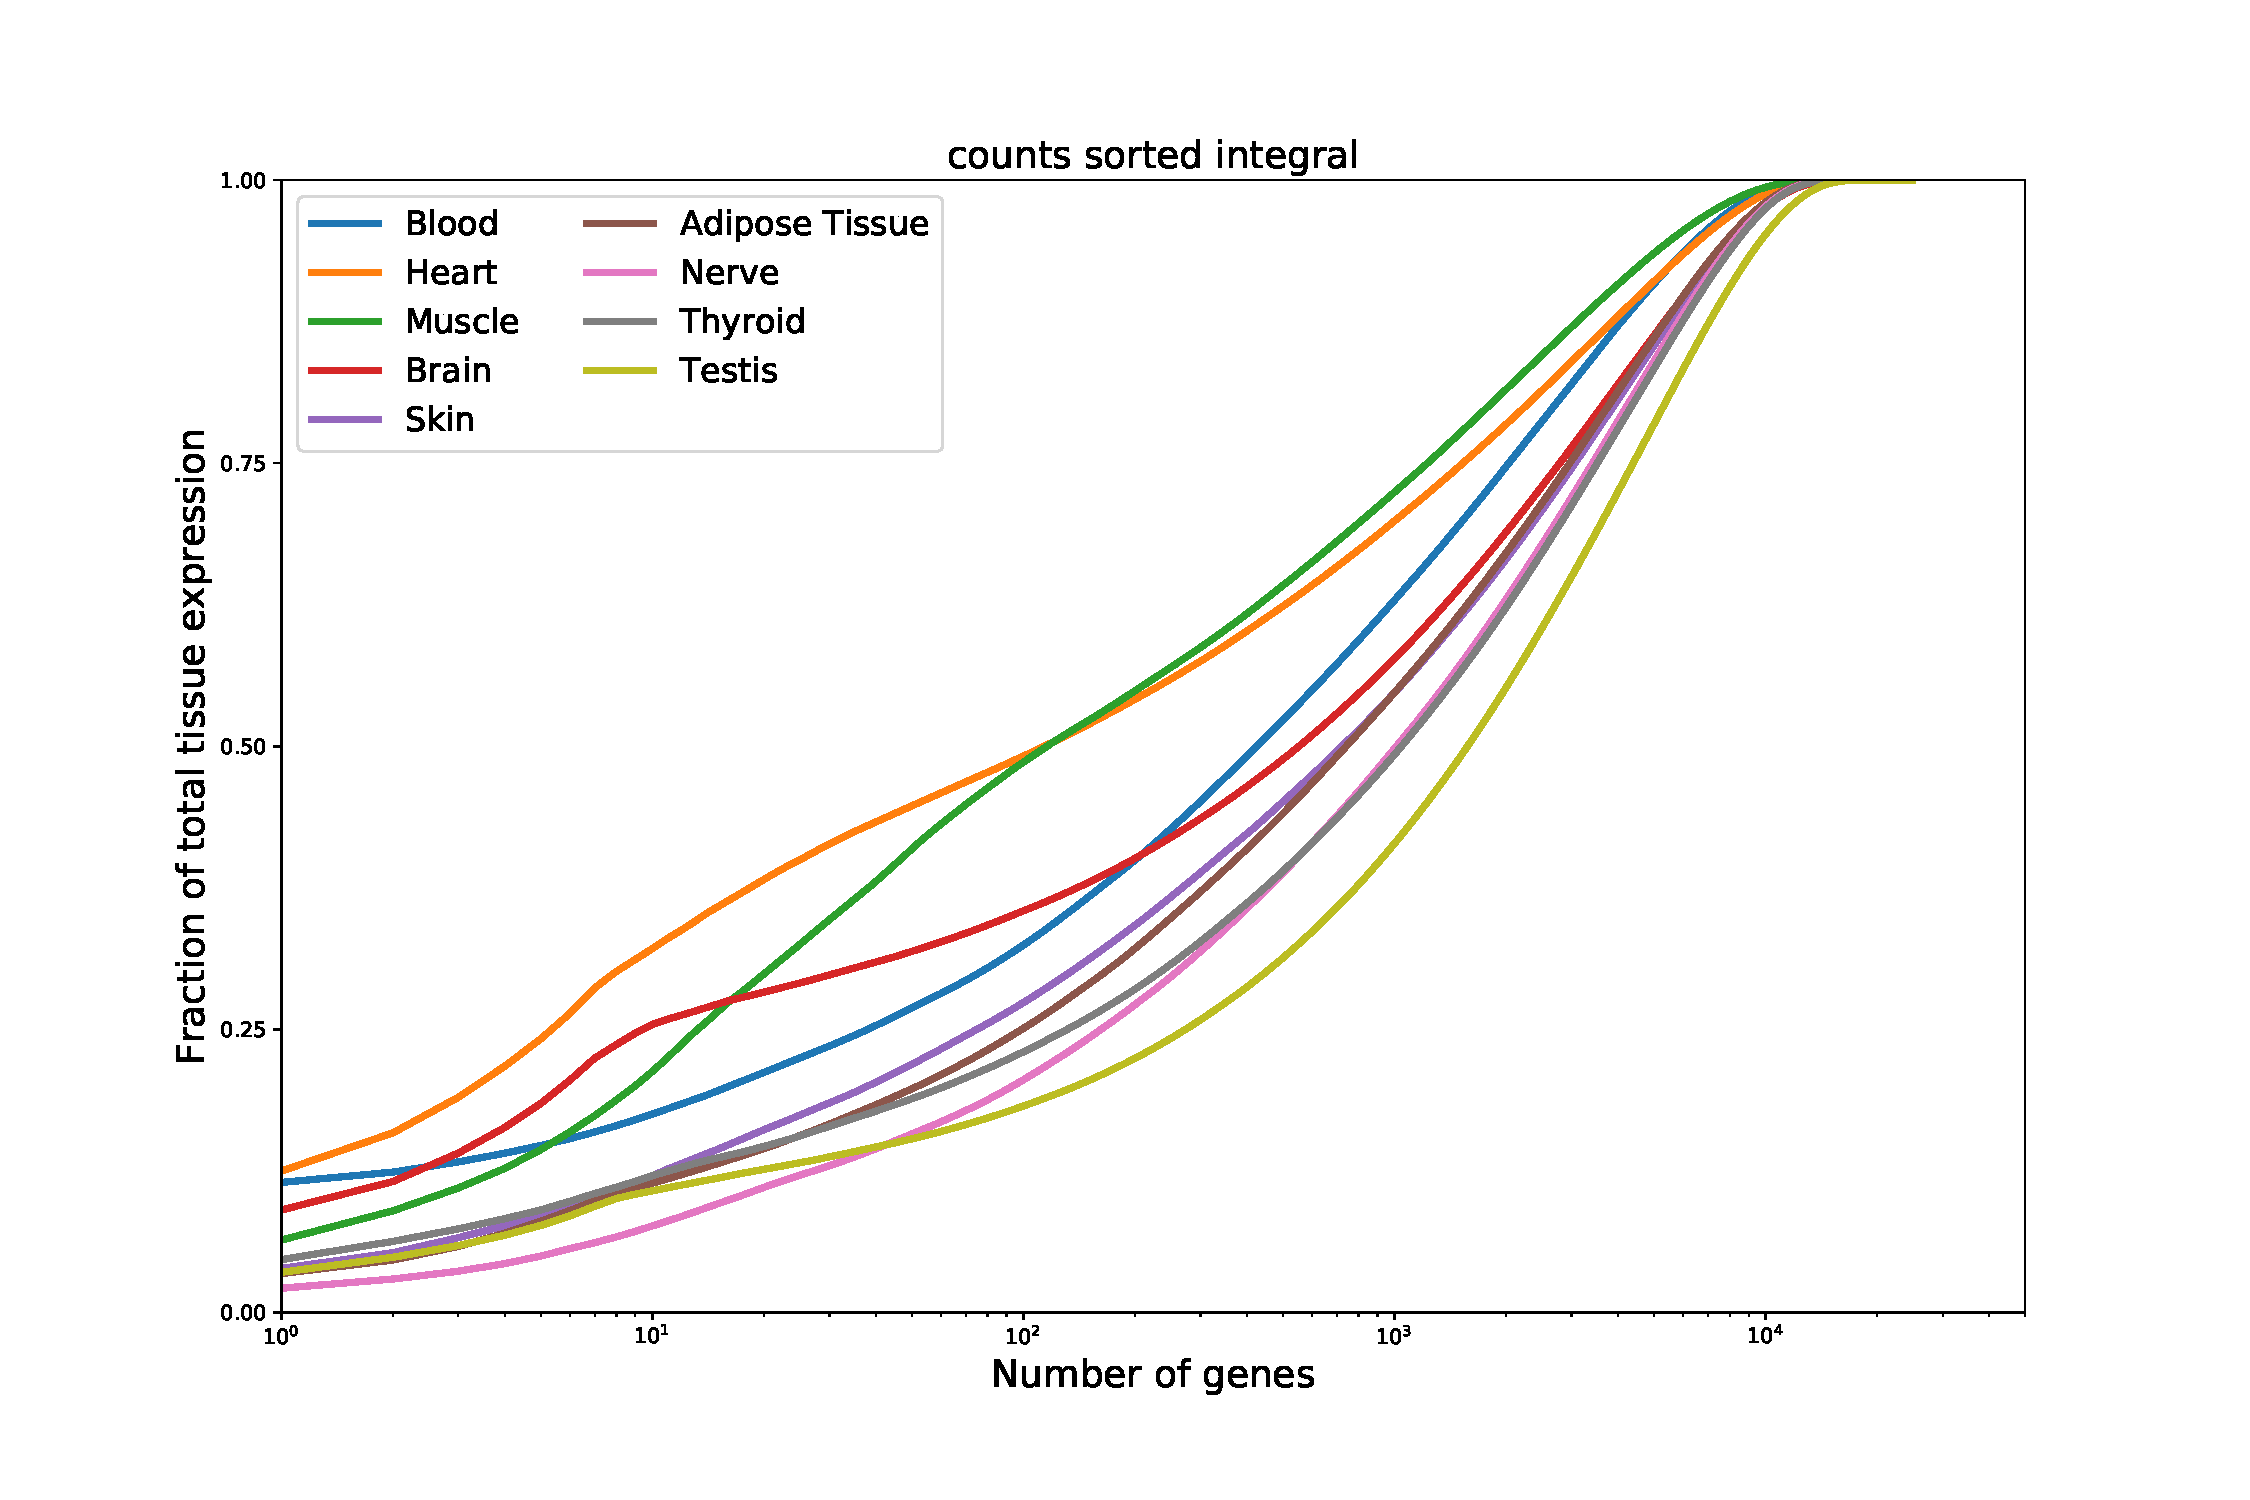
\includegraphics[width=0.9\linewidth]{pictures/structure/gtex/fraction_of_trascriptome.pdf}
  \caption{The integral of the sorted abundances for each tissue.}
  \label{fig:structure/gtex/fraction_of_trascriptome}
\end{figure}
\FloatBarrier
Here, when a curve is steep it means that a few genes' expression represents a great fraction of the total size of the transcriptome. If a curve is smooth it means that many genes are necessary to describe the whole transcriptome for that particular tissue. This analysis shows that different tissues have a different complexity in terms of the number of genes necessary to build the transcriptome (in average). In figure~\ref{fig:structure/gtex/fraction_of_trascriptome_Brain} the same analysis is done for the sub-tissues of brain, also these sub-types present a great separation.
\begin{figure}[htb!]
  \centering
  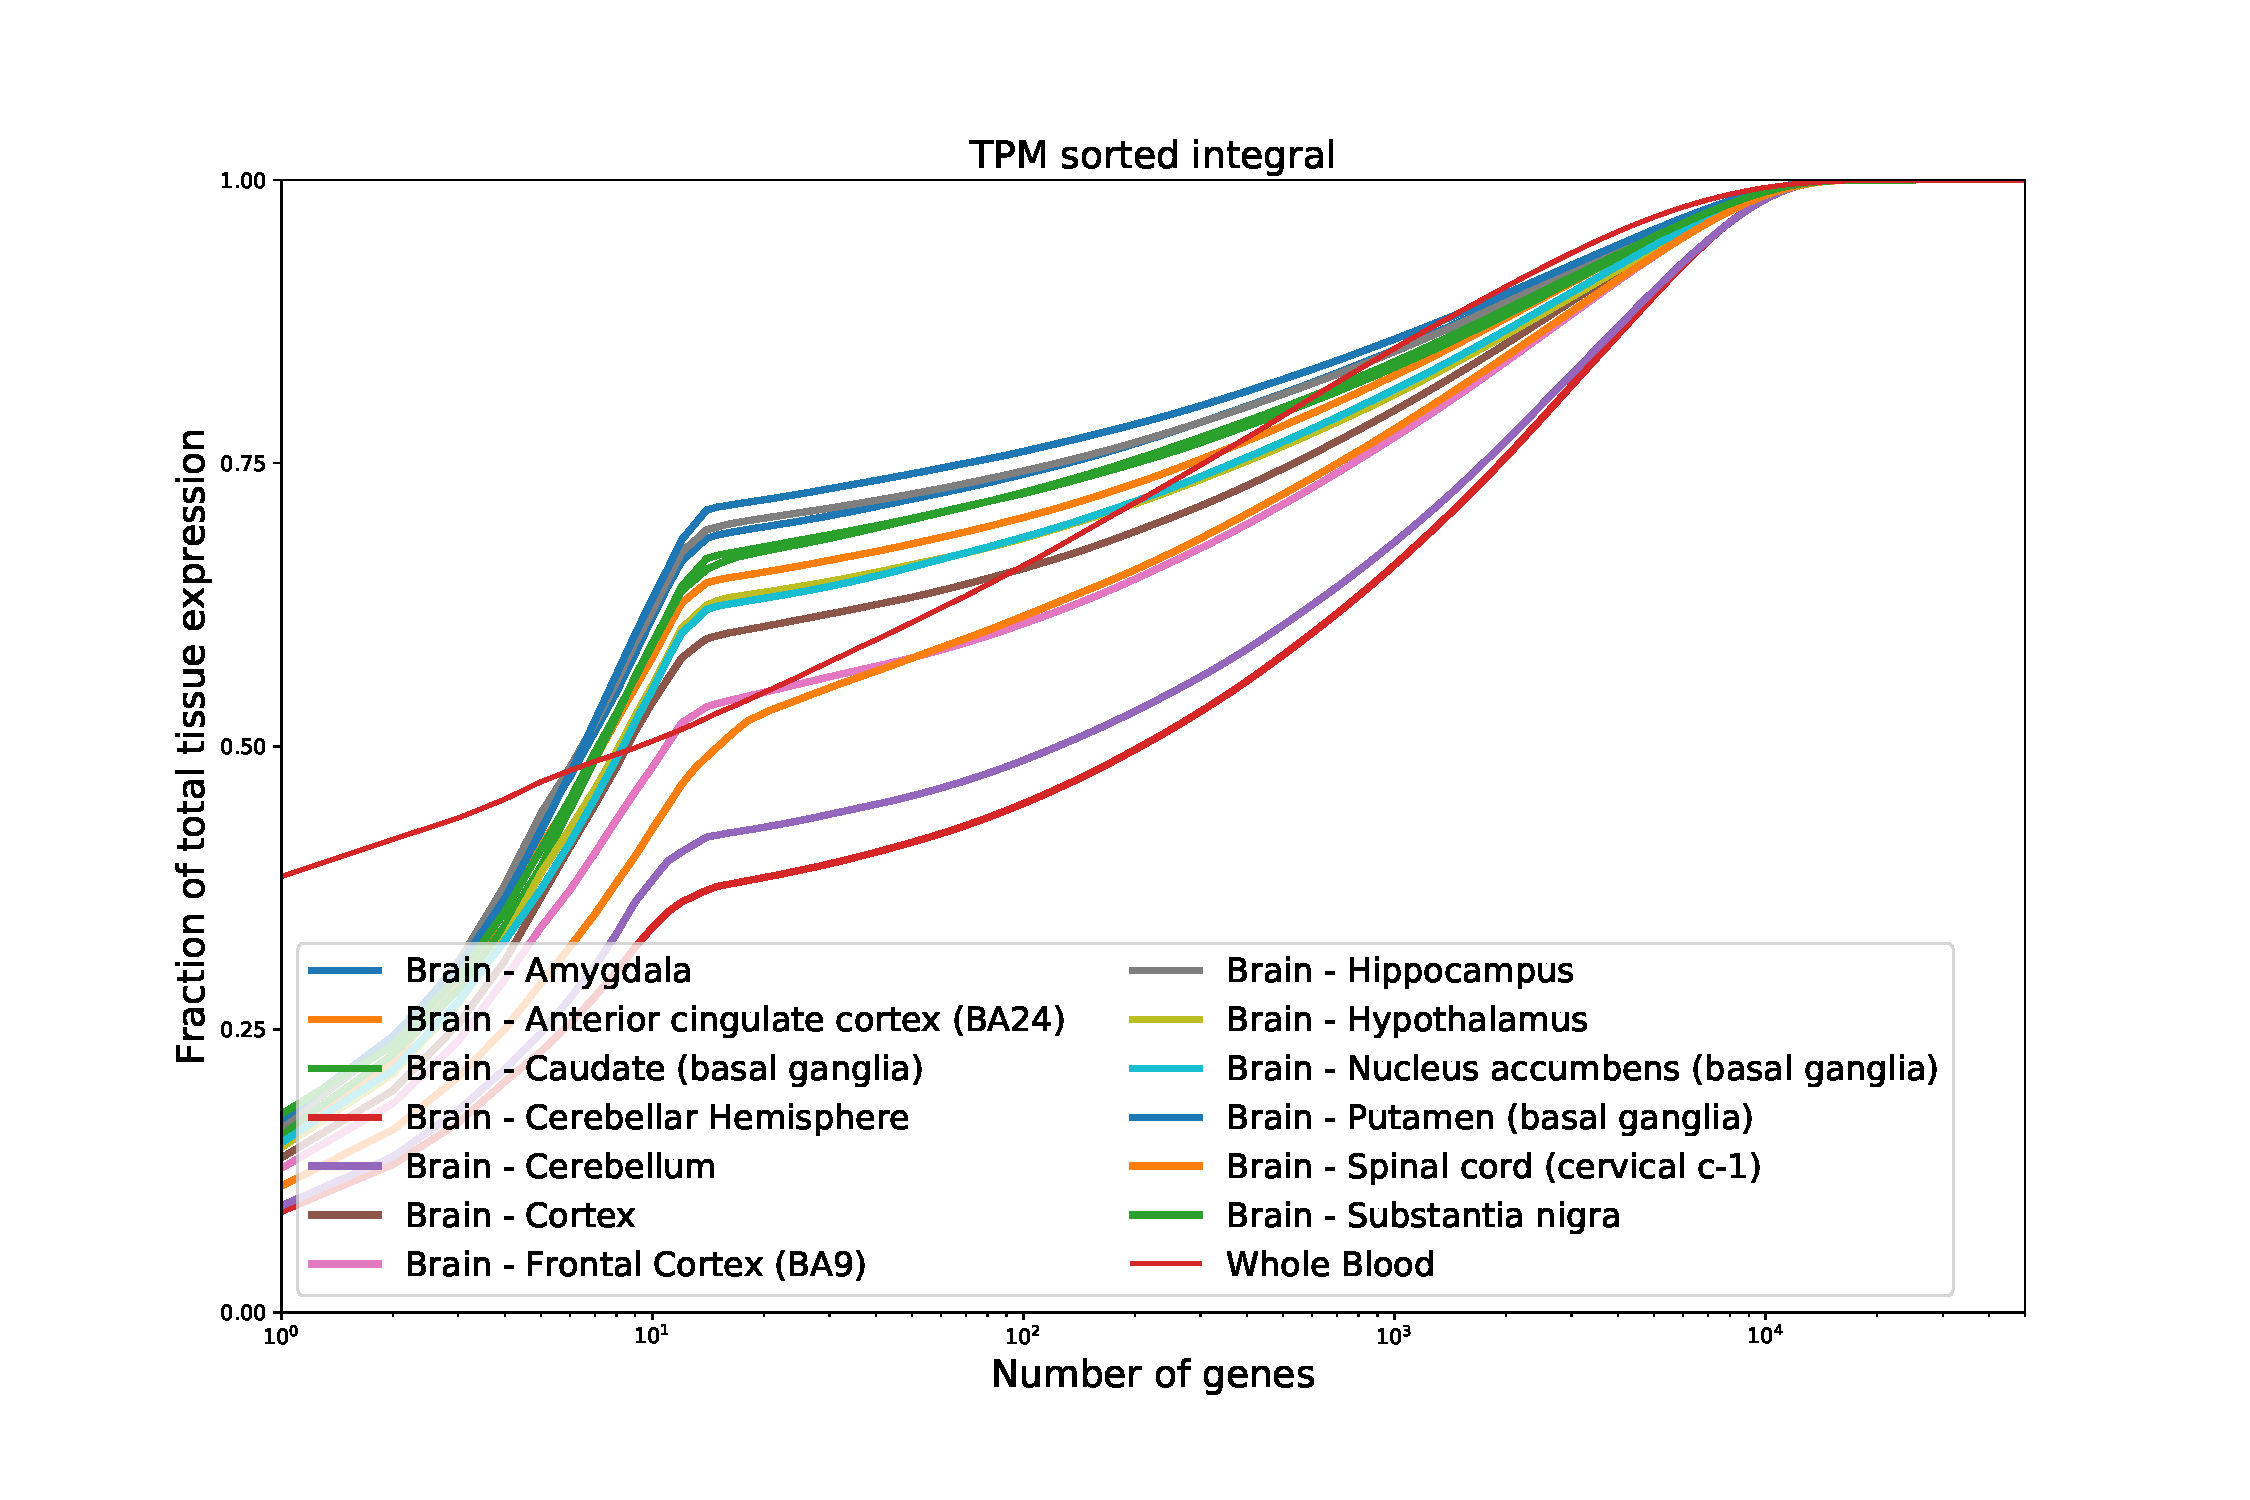
\includegraphics[width=0.85\linewidth]{pictures/structure/gtex/fraction_of_trascriptome_Brain.pdf}
  \caption{The integral of the sorted abundances for sub-types of brain. This is done using TPM to avoid biases due to gene lengths. Blood is plotted for reference.}
  \label{fig:structure/gtex/fraction_of_trascriptome_Brain}
\end{figure}

Another way to interpret this analysis is thinking~\ref{fig:structure/gtex/fraction_of_trascriptome} as the integral of the Zipf's law. So it could be interesting to examine the Zipf's law one tissue a time. In figure~\ref{fig:structure/gtex/zipf_tissue} the Zipf's law for some tissues with an extremal behaviour are reported.
\begin{figure}[htb!]
  \centering
  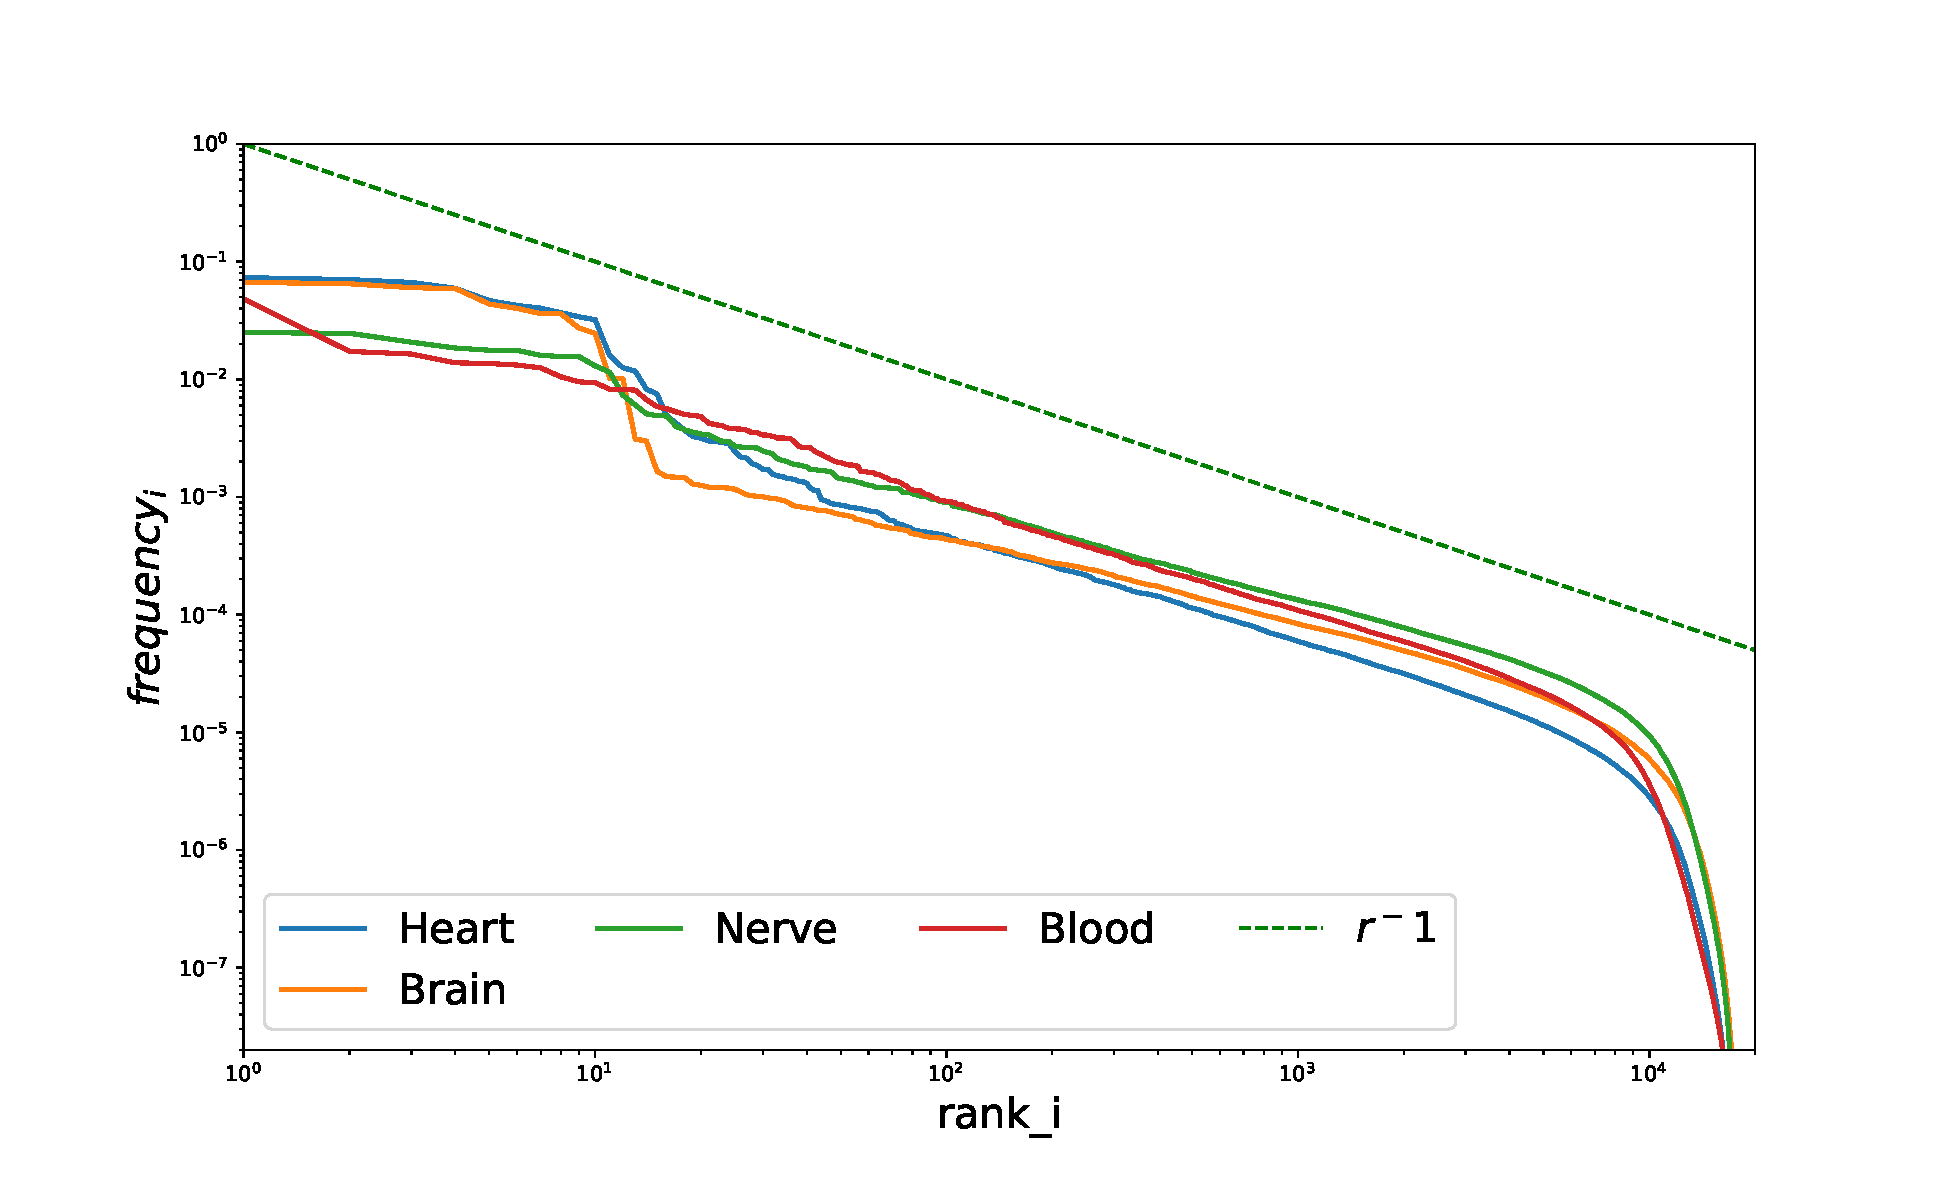
\includegraphics[width=0.8\linewidth]{pictures/structure/gtex/zipf_tissue.pdf}
  \caption{Different tissues present different power law.}
  \label{fig:structure/gtex/zipf_tissue}
\end{figure}
From this point of view, each tissue has its particular slope. The steeper the Zipf the simplest the tissue:. The transcript of a simple tissue can be described with a few genes.
\FloatBarrier
Coming back to the transcriptome analysis. In figure~\ref{fig:structure/gtex/fraction_of_trascriptome} the point where the curve reaches $1$ corresponds to the total number of genes expressed, the remaining ones have a $0$ expression and do not contribute to the transcript. This can be visualized again with the Heaps' law: the number of genes expressed seen in the Heaps' law plot is the number of genes necessary to explain the whole transcriptome. In figure~\ref{fig:structure/gtex/heaps_tissue}, it is evident that there is some kind of tissue differentiation even when looking at the Heaps' law. In other words, two samples with the same size but of different tissues have a different number of genes expressed.
\begin{figure}[htb!]
  \centering
  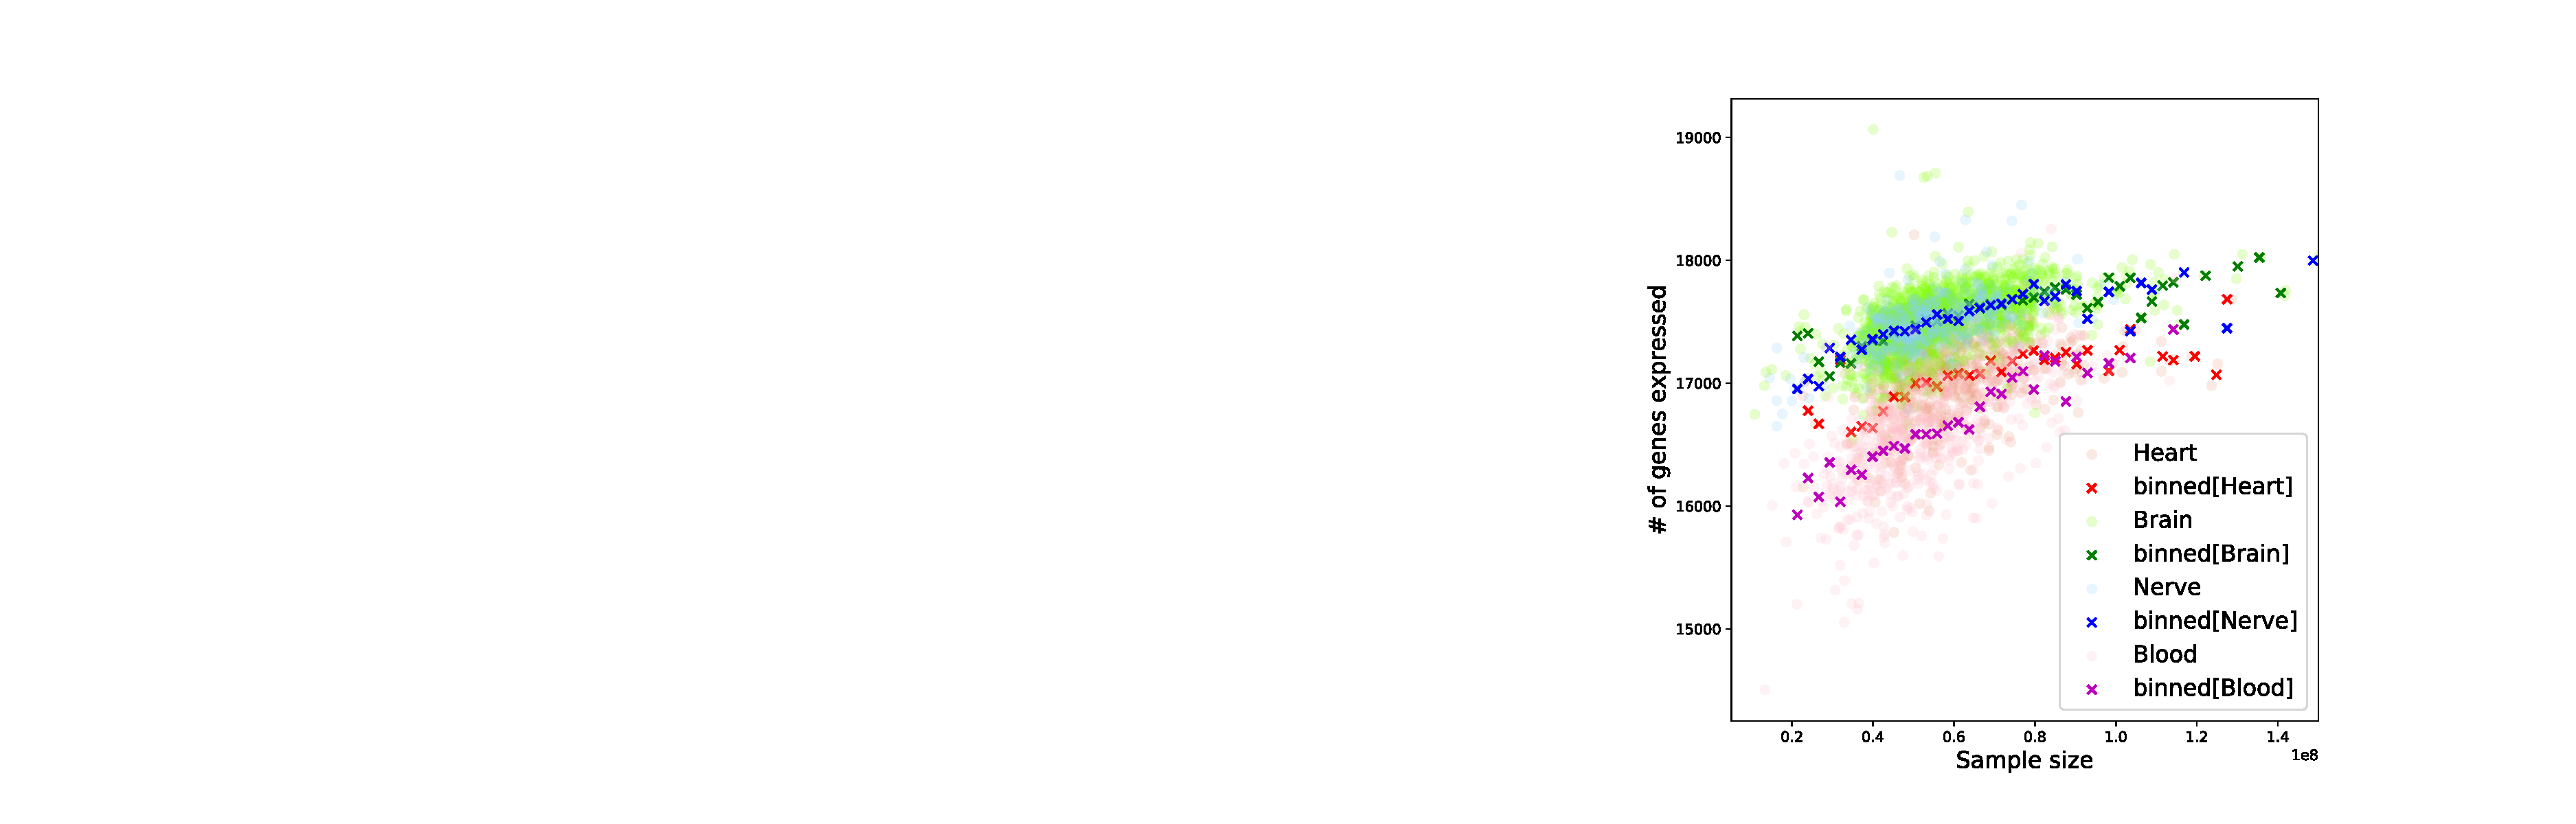
\includegraphics[width=0.5\linewidth]{pictures/structure/gtex/heaps_tissue.pdf}
  \caption{Different tissues express a different number of genes fixed the sample size. This plot was done using counts, using TPM it is not possible because the size on the x-axis is a would be a constant.}
  \label{fig:structure/gtex/heaps_tissue}
\end{figure}
The same analysis can be made by looking at the disease type of cancer samples. In this case, there is no evident differentiation as shown in figure~\ref{fig:structure/tcga/fraction_of_trascriptome_disease}. The only diseases that behave differently are \textit{Parangliomas}, but these are associated only to brain, so the differentiation seen is just a brain separation. This means that separate diseases would be tricky and much more difficult than just separate tissues. The hierarchic approach described in the next chapters will be useful because it is able to separate tissues and disease types at different layers of the hierarchy.
\begin{figure}[htb!]
  \centering
  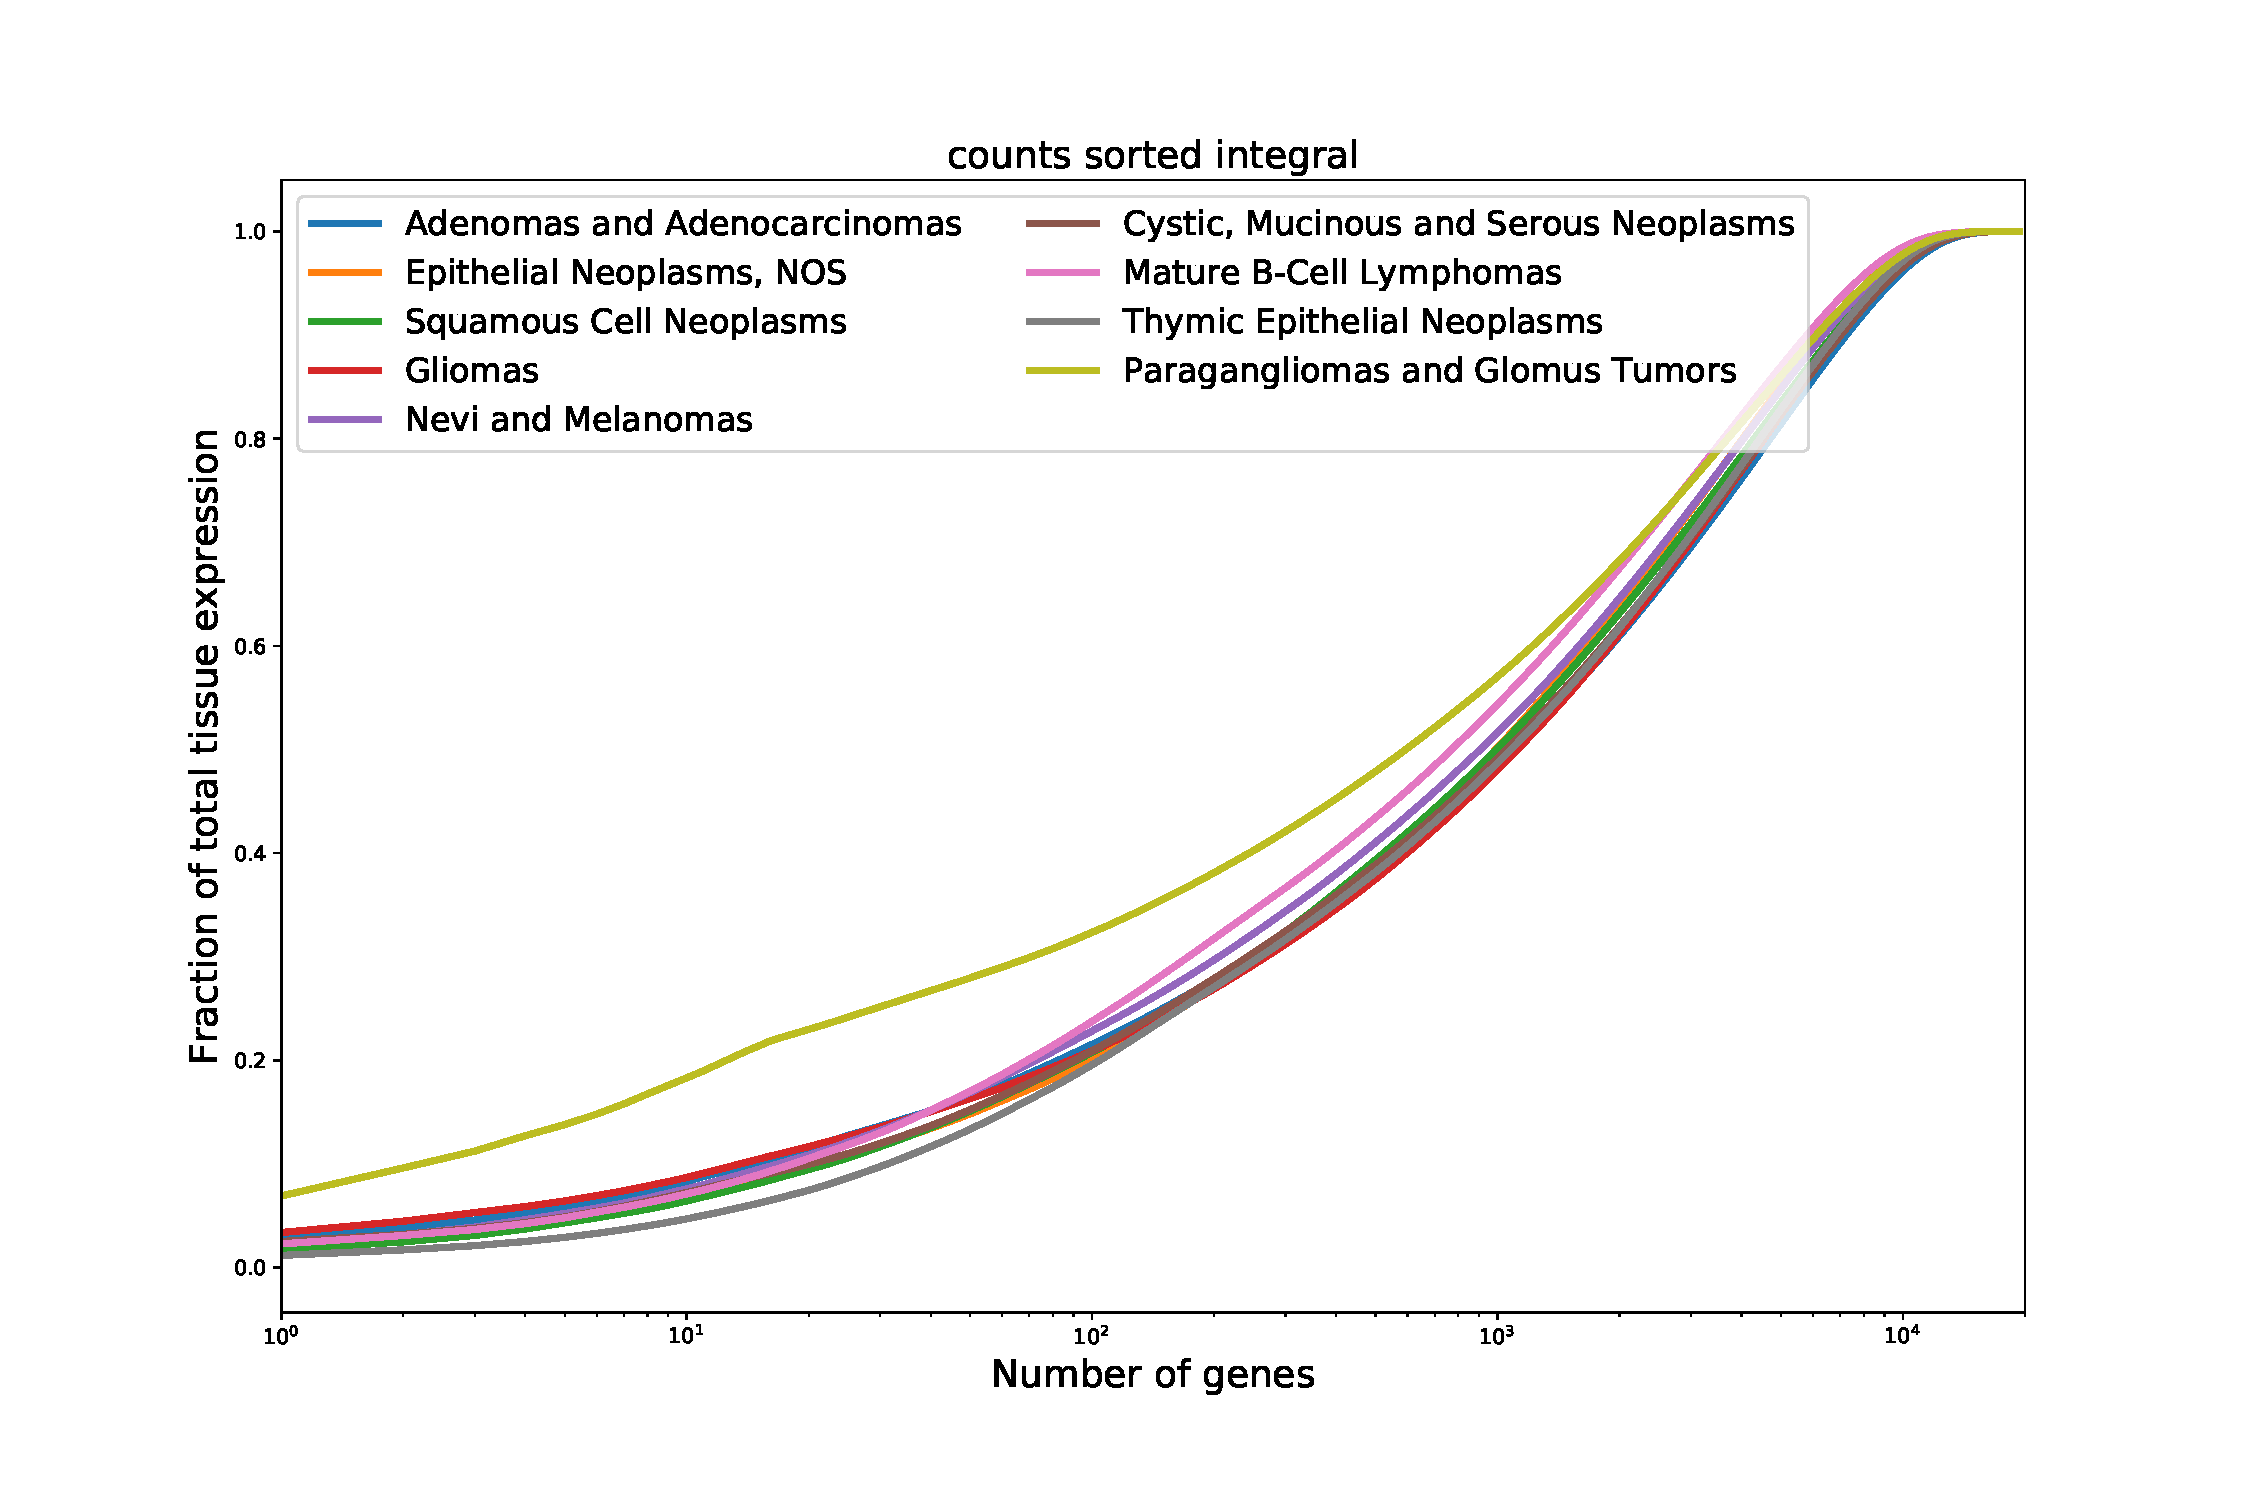
\includegraphics[width=0.8\linewidth]{pictures/structure/tcga/fraction_of_trascriptome_disease.pdf}
  \caption{The integral of the sorted abundances for each disease type.}
  \label{fig:structure/tcga/fraction_of_trascriptome_disease}
\end{figure}

\FloatBarrier
All these analyses suggest that there must be a sort of hidden structure in the data that is somehow related to the tissue each sample comes from. In particular, there are many Zipf's laws hidden behind the data and each sample is build looking at one of these. Moreover, given two samples with a similar size, it happens that the number of genes necessary to build that realization is not always the same (shown by Heaps' law) and it is somehow related to the tissue of the sample.